% \chapter{Introduction}
% The path planning problem is an important application in autonomous systems such as robots and self driving cars \cite{inoue2019robot, gonzalez2016review}. Due to the fact that, nowadays, most physical autonomous systems tasks involve movement from point A to B, it is crucial to find an efficient solution for this problem. As a consequence, we would like to create a path planning decision making algorithm that would plan the journey in such a way that the robot will not collide with any obstacles \cite{gonzalez2016review} in an efficient way.

% But, what is an efficient path planning algorithm? An efficient decision process can refer to multiple aspects such as finding the optimal solution in terms of distance (i.e. shortest distance), most energy efficient solution (robots might have an energy aspect associated with them such as velocity, acceleration, traction power, torque speed that consumes a substantial portion of the battery life) and computational cost (in the real world robots need to process the terrain and take decisions at each point in time, if the algorithm is really slow it could not even reach the destination especially if the environment is constantly moving) \cite{gonzalez2016review}.

% The aim of the paper is to develop such a decision algorithm by using an LSTM \cite{hochreiter1997long} (Long short-term memory) recurrent neural network and compare it to the previous works \cite{nicola2018lstm, lee2018lstm, inoue2019robot}. But in order to correctly asses the performance of the algorithm we need to review the current existing solutions and compare our results against them as well.

% \section{Motivation}
% In the \hyperref[LiteratureReview]{Literature Review} section we are going to study the current available solutions to the path finding problem and the first thing that we are going to notice is that there are a lot of them (not including variations). So why would we bother creating a new algorithm when so many good solutions exist already?

% %\subsection{Importance}
% % - why does it matter
% % - include example, bomb defusing, warehouses Amazon
% % - should be fast, quality
% % - technical aspects
% % - advantages of NN over classic algorithms (uncertainty)
% % - technical objectives
% % - move from A to B

% \section{Proposed method}
% % - talk about the LSTM solution
% The reason of choosing the LSTM approach is because the path planning algorithm can be described as a sequential problem and the LSTM is build with the purpose of solving this kind of problems.

% %\subsection{Significance}
% % - high level (general)
% % - more subjective
% % - repeat importance, but high level

% \section{Outline}
% % - report chapters summarised (2-3)

% \section{Methodology}
% % - how I am going to solve it
% % - image map
% % - network
% % - map generation: game of life

\chapter{Introduction}

Path planners have essential applications in physical autonomous systems, such as robots and self-driving cars, as they have to safely follow an efficient, collision-free trajectory to their destination \cite{inoue2019robot, gonzalez2016review}. Nowadays, autonomous systems are indispensable, their purpose being, the automation of tasks that cannot be performed at large scale or in a safe manner by a human being. Some examples include military applications (e.g. bomb-defusing robots), search-and-rescue robots, large scale manufacturing robots and warehouses management robots \cite{inoue2019robot}. As a consequence, it is crucial to develop an efficient path planning algorithm that would plan a safe journey for the robot \cite{gonzalez2016review}.

We argue that in real-world path planning, the robots interact with the real world environment and thus are subject to physical constraints. Therefore, the path planning decision algorithm has to satisfy various requirements imposed by hardware limitations \cite{lavalle2001randomized}: 

\begin{itemize}
    \item \textbf{Resource Load} - The solution has to be computationally and memory efficient by taking into account the hardware limitations imposed by the robot architecture
    \item \textbf{Partial Knowledge (Online Planners)} - Usually in robotics, the planner has to find a solution with partial knowledge about the map. Thus, the algorithm has to explore the map while searching for a solution (i.e. the algorithm becomes online; e.g. a robot with a SLAM sensor has only localised information, until more areas are discovered)
    \item \textbf{Dynamic Environments} - The real world is highly dynamic and local path planning algorithms should support real-time path generation and collision detection
    \item \textbf{Robustness to Unknown Environments} - The solution should generalise well in unknown environments by preserving all other constraints
    \item \textbf{Non-holonomic Constraints} - Most robots (e.g. self-driving cars) do not possess the ability to move in all available degrees of freedom instantaneously. Therefore, the solution should plan a trajectory that can be followed with maximal efficiency (e.g. a car has to follow a curved path when turning to the left or right). Lastly, the path should also take into consideration the available physical capabilities of the robot (e.g. a robot has limited manoeuvring)
    \item \textbf{Randomized Kinodynamic Planning} - Path planners should generate a path based on the imposed vehicle constraints such as velocity, acceleration and torque. Therefore, we can avoid collisions with obstacles due to high velocity
    \item \textbf{Higher Dimensional Scaling (3D)} - The solution should be easily and feasibly extended to robots with higher degrees of freedom (e.g. drones and flying robots)
\end{itemize}

% real world applications in industry, dynamic environments, robustness, randomized kinodynamic planning, non-holonomic constraints, higher dimensional scaling (3D) and resource load.

% Move in significance
%Nowadays, autonomous systems are indispensable and they serve as purpose, the automation of tasks that can't be performed at large scale or in a safe manner by a human being. Some examples include military applications (e.g. bomb defusing robots), search-and-rescue robots, large scale manufacturing robots and warehouses management robots. As a consequence, it is crucial to develop an efficient path planning decision making algorithm that would plan a safe journey for the robot \cite{gonzalez2016review}.

% But, what is an efficient path planning algorithm? An efficient decision process can refer to multiple aspects such as finding the optimal solution in terms of distance (i.e. shortest distance), most energy efficient solution (robots might have an energy aspect associated with them such as velocity, acceleration, traction power, torque speed that consumes a substantial portion of the battery life) and computational cost (in the real world robots need to process the terrain and take decisions at each point in time, if the algorithm is really slow it might not even reach the destination especially if the environment is constantly moving) \cite{gonzalez2016review}.

Currently, there are a lot of classic solutions to the pathfinding problem. To mention some of the most important ones: A* \cite{choset2005principles, duchovn2014path, zhang2014multiple, 5937169}, Rapidly-exploring Random Tree (RRT) family \cite{lavalle1998rapidly, rodriguez2006obstacle, lavalle2001randomized, karaman2011sampling}, Value Iteration on Markovian Decision Processes (MDP) \cite{szepesvari2010algorithms, satia1973markovian}. However, most of the classic algorithms are computationally expensive because they have to search a vast area. A* and Informed RRT* are pruning the search space by adopting a heuristic function $h$ (e.g. the Euclidean distance between the agent and the goal or the ellipsoid heuristic respectively), but even so, if the environment is complex (e.g. contains unusually shaped obstacles, the path is meandering), the search is not pruned enough. Moreover, the computational cost and memory increase exponentially with the dimension of the environment. Additionally, there exist environments (e.g. maps without a metric space such as networks) where finding a proper heuristic function is not trivial. Lastly, most of the classic algorithms are offline, and thus, they require full knowledge about the map.

\section{Objective}

This project aims to investigate if Machine Learning (ML) methods are a viable option for path planning applications. We will attempt to develop a ML solution that solves the path planning problem while satisfying the real world industrial applications requirements. We are going to focus mainly on the partial knowledge, resource load reduction (memory efficiency; See Figure \ref{fig: intro_show}) and robustness to unknown environments properties by running empirical evaluations while only theoretically prove the others.

The proposed solution will be developed using an LSTM \cite{hochreiter1997long} (Long Short-Term Memory) recurrent neural network architecture. The motivation behind choosing an LSTM architecture is derived by the fact that the path planning algorithm can be described as a sequential problem and it has been proved that LSTMs produce excellent results in this area (e.g. speech recognition, time series, anomaly detection, text generation, machine translation and many more) \cite{Goodfellow-et-al-2016}. There has been some work done with LSTMs \cite{nicola2018lstm, lee2018lstm, inoue2019robot} in this field, but their approach had a low success rate of finding a path to the goal (even if one exists). Therefore, we will attempt to boost the success rate by creating hybrid solutions between pure ML solutions and classic solutions such as A*.

In order to achieve the objectives mentioned above, we are going to use a simulation platform. Currently, there are a variety of standardised motion planning libraries such as: \textit{ROS} \cite{Quigley09}, \textit{OMPL} \cite{sucan2012the_open_motion_planning_library}, \textit{MoveIt} \cite{moveit} (which has benchmarking capabilities \cite{moll2015benchmarking}). However, we are going to build our development platform, PathBench. The main reason behind this choice is that we are going to focus on the actual generation of the path instead of the physical interactions between the robot and the environment. Thus, we boost development productivity while focusing on the key components of the solution. Furthermore, by creating standardised APIs, we can easily port the path planners to the specified libraries. Finally, we need training data, a ML pipeline and a benchmarking module which the current libraries do not provide.

\begin{figure}[h!]
  \centering
  \begin{subfigure}[b]{0.32\linewidth}
    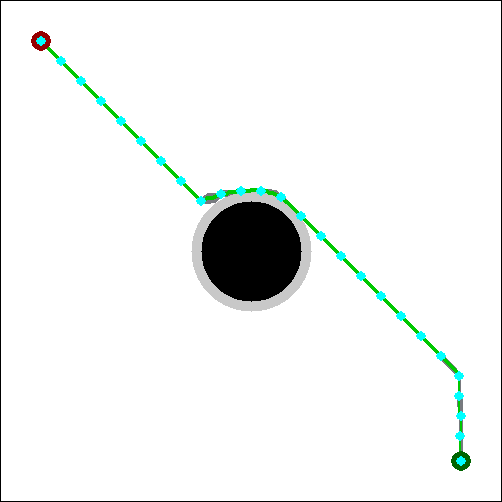
\includegraphics[width=\linewidth]{images/screenshot_51.png}
    \caption{Global Way-point LSTM Planner (proposed solution)}
  \end{subfigure}
  \hspace{2cm}
  \begin{subfigure}[b]{0.32\linewidth}
    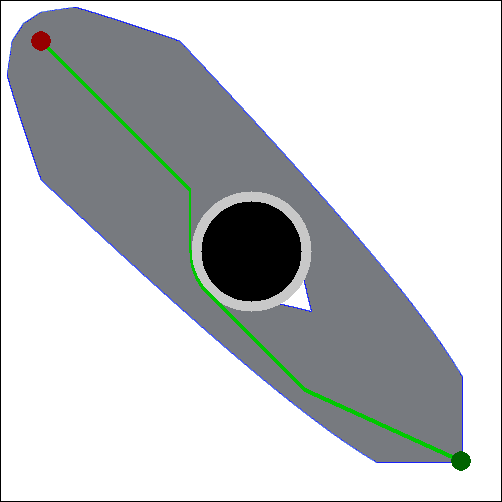
\includegraphics[width=\linewidth]{images/screenshot_44.png}
    \caption{A* \newline}
  \end{subfigure}
  \caption{Memory load comparison between the Global Way-point LSTM Planner (proposed solution) and A*. The red circle represents the agent (robot) position, the green circle represents the goal position and the black/light-grey regions represent obstacles. The dark grey regions represent the total search space used by the respective algorithms}
  \label{fig: intro_show}
\end{figure}

\pagebreak

% Tare goinhe aiuse a simulation platform. Currently, there are a variety of m, g to we  of the report, is to develop a pruning algorithm that will speed up a classic algorithm such as A* or Informed RRT* by reducing the search space.

% Having this in mind, we are going to use an LSTM \cite{hochreiter1997long} (Long short-term memory) recurrent neural network architecture to implement the above mentioned procedure by using A* as ground truth. There has been some work done with LSTMs \cite{nicola2018lstm, lee2018lstm, inoue2019robot}, but their approach was to use LSTMs to \textbf{produce} an actual path. One of the major disadvantages of using this method, is that the robot will not always succeed in finding the goal, even if there \textbf{exists} a solution \cite{nicola2018lstm}. Therefore, we introduce the idea of probabilistic search space, in order to make sure that the algorithm will eventually find a path.

% The reason of choosing an LSTM architecture is derived by the fact that the path planning algorithm can be described as a sequential problem and it has been proved that LSTMs produce great results in this area (e.g. speech recognition, time series anomaly detection, text generation and many more).

% Moreover, by using a machine learning approach we should solve the problem of finding a good heuristic function in complex environments.

%\section{Significance}
%We argue that in real world path planning, the robots interact with the real world environment and thus are subject to physical constraints. Therefore, we attempt to develop a solution that solves some of the following areas: real world applications in industry, dynamic environments, robustness, randomized kinodynamic planning, non-holonomic constraints, higher dimensional scaling (3D) and resource load.

%\todo{Complete this section}

%In order to devise an extension for a current solution, we first need to study the current available classic algorithms which are eligible with this kind of extension. We will also cover the non-eligible algorithms as a comparison standard. The \hyperref[LiteratureReview]{Literature Review} section presents the most popular classic path finding algorithms.

%In the \hyperref[Background]{Background} section, we are going to review the machine learning architectures and principles needed in the development of the proposed solution.

%In the \hyperref[Solution]{Solution} section, we are going to state our proposed solution by exemplifying the machine learning architecture that we have used and the algorithm itself.

%In the \hyperref[Simulator]{Simulator} section, we are going to discuss about our simulation environment where we will be testing the proposed solution and generate the training data.

%In the \hyperref[Evaluation]{Evaluation} section, we are going to asses the performance of the proposed solution against the studied algorithms.

%In the \hyperref[Conclusion]{Conclusion} section, we are going to summarise our findings and address future work.

\section{Contributions}

The contributions of this report include (the source code can be found at \url{https://gitlab.doc.ic.ac.uk/ait15/individual-project}): 

\begin{itemize}
    \item Three algorithmic contributions: \begin{itemize}
        \item \textbf{CAE Online LSTM Planner} - The first proposed solution, Online LSTM Planner, is almost identical to the paper implementation from \cite{nicola2018lstm} with different input selection and the addition of a max iterations argument. The CAE Online LSTM Planner is a hybrid solution between \cite{nicola2018lstm} and \cite{inoue2019robot}. The Convolutional Auto-encoder (CAE) architecture was built by us, and the LSTM architecture was borrowed from \cite{nicola2018lstm}
        \item \textbf{LSTM Bagging Planner} - This algorithm is inspired by ensemble learning solutions, and it is used to boost the performance of the Online LSTM and CAE Online LSTM Planners
        \item \textbf{Global Way-point LSTM Planner} - The final proposed solution uses the LSTM Bagging Planner to create a global way-point suggestion algorithm. It has nice flexibility properties, significantly reduced memory load compared to A*, support for partial knowledge environments, robustness to unknown environments and a theoretically lower average case time and space complexity compared to A*
    \end{itemize}
    \item PathBench - A benchmarking platform for classic and learned path planning algorithms with the following four main components and extension: 
    \begin{itemize}
        \item \textbf{Simulator} - We have built a simulator as a practical way of visualising the behaviour of the path planners. It includes different features such as animations, control for animations (stop, resume), custom displays for individual algorithms and it is highly extensible to support new solutions
        \item \textbf{Generator} - The generator was build to acquire training data for our ML solutions. It can generate three types of maps: uniform random fill maps, block maps and house maps. It can also be extended to include more synthetically generated data (e.g. cellular automata cave generation and maze generation) as well as convert real-world datasets (e.g. Simultaneous Localisation and Mapping (SLAM) images \cite{dissanayake2001solution}) into internal simulator environments. All maps can be converted into training datasets which contain a variety of features and labels generated using A* as ground truth
        \item \textbf{Trainer} - We have built a training environment to boost the productivity of testing new ML architectures. It has an automatic pipeline for extracting a subset of the generated training data and caching subroutines to increase the speed of second runs
        \item \textbf{Analyser} - We have developed an analyser tool to assess the performance of the proposed algorithms against classical solutions such as A*. The analyser contains multiple assessment routines which stress the performance of the tested algorithms in multiple areas (e.g. speed, efficiency and memory)
        \item \textbf{ROS Real-time Extension} - We have added support for real-world simulation by implementing an updatable map environment which is compatible with the \textit{gmapping} \textit{ROS} package (i.e. SLAM scan)
    \end{itemize}
    \item Theoretic and real-world evaluations performed as follows: \begin{itemize}
        \item \textbf{Complexity and Theoretical Analysis} - For each proposed solution, we have theoretically proven the worst case time and space complexity. Moreover, we have discussed the worst case time and space complexity of higher dimensional scaling. Lastly, we have proved that the proposed solution achieves theoretically lower average case time and space complexity compared to A*
        \item \textbf{Empirical Methods} - We have created specific statistical metrics for each proposed solution. The metrics are used to gain insight into the general behaviour of the proposed solutions and their real-world applications effectiveness. We have showed that the proposed solution significantly reduces the memory load compared to A* (See Figure \ref{fig: intro_show}) and that it generalises well in unknown environments
        \item \textbf{Real-world Evaluation} - We have tested the performance of the proposed solution on real-world occupancy grid maps generated by real-world robots. Furthermore, we have implemented the proposed solution on a real-world robot and tested it at Imperial College London. We have proved that the proposed solution is applicable in real-world scenarios. Moreover, we have proved the partial knowledge property by showing that the algorithm can run in environments with partial information in which some classic offline algorithms such as A* are unable to find a solution
    \end{itemize}
\end{itemize}

\section{Report Outline}
%\textbf{\hyperref[LiteratureReview]{Literature Review}.}
%\paragparh{Chapter \ref{LiteratureReview} (\hyperref[LiteratureReview]{Literature Review}).}
\paragparh{\hyperref[LiteratureReview]{Literature Review} (Chapter \ref{LiteratureReview}).} In this chapter, we will study the current path planning solutions by categorising them into separate sections based on the type of planner. We will assess the optimality conditions, give a brief time and space complexity analysis, study the structure of the algorithms and state the advantages and disadvantages of each solution.

% \textbf{\hyperref[Background]{Background}.}
%\paragparh{Chapter \ref{Background} (\hyperref[Background]{Background}).}
\paragparh{\hyperref[Background]{Background} (Chapter \ref{Background}).} The Background Chapter will cover the basics of ML and explain the structure of the LSTM network. We will discuss data pre-processing, training routines, evaluation methods and hyper-parameter tuning.

% PathBench
% MLWP Planner
% capital section

%\textbf{\hyperref[Simulation Platform]{Simulation Platform}.} 
%\paragparh{Chapter \ref{Simulation Platform} (\hyperref[Simulation Platform]{Simulation Platform}).} 
\paragparh{\hyperref[Simulation Platform]{PathBench} (Chapter \ref{Simulation Platform}).} In this chapter, we are going to describe PathBench, the platform used to develop and test the classic and proposed solutions. We will cover the architecture design of all platform components and explain the current capabilities and limitations by comparing it to the standard motion planning libraries.

%\textbf{\hyperref[sec: methods]{Methods}.}
%\paragparh{Chapter \ref{sec: methods} (\hyperref[sec: methods]{Methods}).}
\paragparh{\hyperref[sec: methods]{Methods} (Chapter \ref{sec: methods}).} In this section, we are going to describe the proposed solutions by following the same investigations as in Chapter \ref{LiteratureReview} (\hyperref[LiteratureReview]{Literature Review}). Moreover, we will compare the theoretical performance against the well-known algorithm A* by giving a thorough time and space complexity analysis for all proposed solutions.

%\textbf{\hyperref[Evaluation]{Evaluation}.} 
%\paragparh{Chapter \ref{Evaluation} (\hyperref[Evaluation]{Evaluation}).} 
\paragparh{\hyperref[Evaluation]{Evaluation} (Chapter \ref{Evaluation}).} In this chapter, we are going to run a series of empirical evaluation routines which will stress the proposed solution performance. We are going to examine each empirical run and give a theoretical interpretation of the results. Moreover, we will test the performance of the path planner on real-world occupancy grid maps produced by real-world robots. Lastly, we will run the proposed solution on a real robot at Imperial College London and assess its performance.

%\textbf{\hyperref[Conclusion]{Conclusion}.} 
%\paragparh{Chapter \ref{Conclusion} (\hyperref[Conclusion]{Conclusion}).} 
\paragparh{\hyperref[Conclusion]{Conclusion} (Chapter \ref{Conclusion}).} In the final chapter, we are going to summarise our findings and address future work.